\documentclass[11pt]{article}

\usepackage[margin=1in]{geometry}
\usepackage{booktabs}
\usepackage{float}
\usepackage{amsmath}
\usepackage{amssymb}
\usepackage{array}
\usepackage{graphicx}
\usepackage{xcolor}
\usepackage{tikz}
\usepackage[hidelinks]{hyperref}
\usepackage[numbers,sort&compress]{natbib}
\usetikzlibrary{arrows.meta,positioning}
\newcolumntype{L}[1]{>{\raggedright\arraybackslash}p{#1}}

\title{IAD-Risk: Risk-Aware Identity-Agenda Disentanglement for Scholarly Work Deduplication}
\author{Anonymous Authors}
\date{}

\begin{document}
\maketitle

\begin{abstract}
Scholarly entity matching must distinguish whether two records describe the same work, not merely whether they discuss the same research agenda. Modern scientific representations and pair classifiers often improve semantic matching, but a high semantic score can also connect different papers in the same task, benchmark, or citation community. This paper studies this failure mode as \emph{identity-agenda confusion} and proposes IAD-Risk, a risk-aware framework that separates identity evidence from agenda evidence before making merge decisions. IAD-Risk combines stratified data provenance, identity and agenda relation heads, and false-merge risk gating to prevent agenda-level hard negatives from entering automatic merge clusters. We evaluate the framework with IAD-Bench, a benchmark contract that separates DeepMatcher gold labels, SciRepEval/SciDocs-style proxy labels, and OpenAlex/OpenCitations silver hard negatives. On IAD-Bench-Open-v2, transformer-backed IAD-Risk variants retain high same-work performance while reducing hard-negative false merges that affect single-space scientific representation baselines. The results support a conservative conclusion: identity-agenda disentanglement is a practical mechanism for safer scholarly deduplication, while additional manual validation and broader source-heldout validation remain necessary before making broad method-ranking claims.
\end{abstract}

\section{Introduction}

Scholarly knowledge systems rely on entity matching to decide whether multiple records describe the same scientific work. Digital libraries, literature review tools, citation graphs, recommender systems, and evidence synthesis pipelines all require stable work identities because a false merge can combine evidence from different papers and distort downstream analysis. This paper focuses on scholarly work deduplication: given two scholarly records with titles, abstracts, authors, venues, identifiers, topics, and citations, the system must decide whether the records can be safely merged as the same work.

The central challenge is that topical similarity is not identity evidence. Two papers can share a task, dataset, method family, citation neighborhood, or OpenAlex topic while making different contributions. Scientific representation models such as SPECTER and SciNCL are valuable because they bring related papers close in embedding space \citep{cohan2020specter,ostendorff2022scincl}, but the same behavior can create false-merge risk when a deduplication system treats semantic closeness as work identity. This failure is particularly important in scholarly settings because false merges are harder to repair than missed duplicates: once distinct papers are clustered as one work, citation counts, recommendation signals, and review evidence can be contaminated.

We formulate this failure mode as identity-agenda confusion. Identity refers to whether two records denote the same scholarly work. Agenda refers to whether two records discuss the same research problem, benchmark, method family, or citation community. Existing entity matching methods \citep{fellegi1969record,mudgal2018deep,li2020ditto} typically optimize pair classification, while scholarly document representation methods optimize semantic relatedness. Neither objective alone forces the model to learn that same-agenda pairs can be high-risk non-identities.

We propose IAD-Risk, a risk-aware identity-agenda disentanglement framework for scholarly work deduplication. IAD-Risk learns separate relation signals for same-work identity, same-agenda relatedness, and agenda-non-identity hard negatives, then derives a false-merge risk score from these signals. A pair is eligible for automatic merging only when identity evidence is sufficiently strong and agenda-non-identity risk remains below a merge threshold. This selective decision rule turns deduplication from a high-recall similarity problem into a risk-calibrated safety problem.

The paper makes three contributions. First, it defines identity-agenda confusion as a targeted failure mode in scholarly entity matching and introduces hard-negative false-merge rate as a safety metric. Second, it presents IAD-Bench, a provenance-aware benchmark contract that keeps gold, proxy, silver, LLM-silver, and human-reviewed labels separate. Third, it evaluates IAD-Risk under the same pair contract used by representation and entity-matching baselines, while keeping additional LLM and clustering interfaces as reproducible extensions rather than unsupported primary evidence. The current evidence supports targeted false-merge suppression under stratified evaluation; it does not support a broad method-ranking claim or a claim that silver labels replace human gold.

\section{Related Work}

Entity matching and record linkage provide the classical foundation for deciding whether records refer to the same real-world entity \citep{fellegi1969record}. Deep learning methods have extended this line by learning pair representations and matching functions from labeled examples \citep{mudgal2018deep,li2020ditto}. Transformer pair encoders such as RoBERTa \citep{liu2019roberta} provide a practical implementation of this pair-classification paradigm. These systems are strong baselines for scholarly deduplication, but their standard formulation usually treats each pair as a same-entity classification problem and does not explicitly model agenda-level hard negatives or label-provenance boundaries.

Scientific document representation methods learn embeddings that capture citation, topical, and semantic relatedness. SPECTER uses citation-informed supervision to learn document-level representations and introduced SciDocs as a document-level evaluation benchmark \citep{cohan2020specter}. SciNCL further improves scientific representations with neighborhood contrastive learning \citep{ostendorff2022scincl}, and SciRepEval broadens scientific representation evaluation across multiple task formats while releasing the SPECTER2 model family \citep{singh2022scirepeval}. These methods are appropriate baselines because they capture scientific relatedness, yet their strength is also a risk for deduplication: a representation that intentionally brings related papers close can over-connect papers that share an agenda but are not the same work.

Scientific language resources and open corpora make it possible to build reproducible scholarly NLP systems at scale. SciBERT shows that domain-specific pretraining on scientific text improves scientific NLP tasks \citep{beltagy2019scibert}, while S2ORC provides a large open corpus with metadata, abstracts, references, and full text for many open-access papers \citep{lo2019s2orc}. These resources motivate the use of scientific text and citation signals in scholarly matching, but they do not by themselves distinguish work identity from topical relatedness.

Open scholarly metadata sources enable reproducible benchmark construction, but their signals must be interpreted carefully. OpenAlex provides a large open index of scholarly works and concepts \citep{priem2022openalex}, and OpenCitations provides open citation data \citep{heibi2019opencitations}. These sources are useful for constructing agenda-level hard negatives through shared topics or references. However, such labels are silver evidence, not human gold. IAD-Bench therefore treats data provenance as part of the experimental protocol rather than as bookkeeping.

\section{Problem Formulation}

Let $d_i$ and $d_j$ be two scholarly records. The target identity label $y^{I}_{ij}$ indicates whether the records describe the same scholarly work. The agenda label $y^{A}_{ij}$ indicates whether the records discuss a related research agenda. A hard negative is a pair with high agenda evidence but negative identity evidence:
\[
y^{A}_{ij}=1,\quad y^{I}_{ij}=0.
\]
This pair should not be merged even if the documents are semantically close.

We evaluate merge safety with hard-negative false-merge rate:
\[
\mathrm{HNFMR} = \frac{\#\{(i,j): \hat{m}_{ij}=1, y^{A}_{ij}=1, y^{I}_{ij}=0\}}{\#\{(i,j): y^{A}_{ij}=1, y^{I}_{ij}=0\}},
\]
where $\hat{m}_{ij}$ is the automatic merge decision. The goal is not only to maximize same-work F1, but also to control HNFMR under explicit evidence provenance.

\section{IAD-Bench}

IAD-Bench is a benchmark contract for organizing scholarly pair evidence. It is not a claim that every label has the same evidential status. Each pair stores relation labels, expected identity labels, expected agenda labels, label source, label strength, provenance, split, and hard-negative level.

\begin{table}[H]
\caption{IAD-Bench label layers. Gold, proxy, and silver labels are reported separately to avoid overstating evidence strength.}
\label{tab:label-layers}
\centering
\small
\begin{tabular}{lll}
\toprule
Layer & Source & Use in this paper \\
\midrule
Gold & DeepMatcher / py\_entitymatching & Same-work identity evaluation \\
Proxy & SciRepEval / SciDocs-style proximity & Same-agenda analysis \\
Silver & OpenAlex / OpenCitations & Agenda-non-identity hard negatives \\
LLM-silver & LLM pair judgments & Auxiliary analysis and baseline \\
Manual validation & Planned human review & Future validation \\
\bottomrule
\end{tabular}
\end{table}

The Open-v2 benchmark variant used in the core evidence combines 415 DeepMatcher gold pairs with 10,000 OpenAlex-derived silver hard negatives, producing 10,415 pair records over 1,737 documents. The DeepMatcher component provides same-work gold labels, while the OpenAlex component stresses same-agenda non-identity behavior. This design is intentionally conservative: OpenAlex and OpenCitations are used to expose false-merge risk, not to replace human gold.

\section{Method}

\subsection{Overview}

IAD-Risk converts scholarly deduplication into selective risk-aware matching. Given a candidate pair, the model estimates identity, agenda, and agenda-non-identity signals, then derives a false-merge risk score. The final merge decision is made only when identity evidence exceeds a same-work threshold and risk evidence remains below blocking thresholds. Figure~\ref{fig:iad-risk-pipeline} summarizes the workflow.

\begin{figure}[H]
\centering
\small
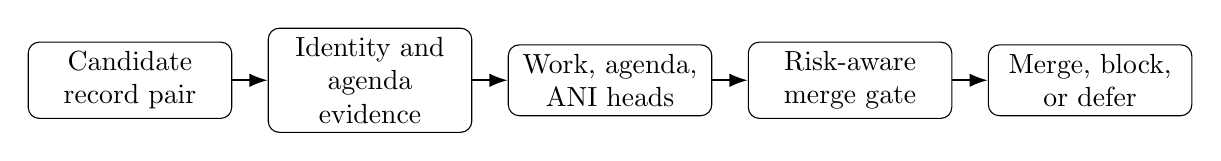
\begin{tikzpicture}[
  node distance=0.45cm,
  box/.style={draw, rounded corners, align=center, minimum height=0.8cm, text width=2.35cm},
  arrow/.style={-Latex, thick}
]
\node[box] (pair) {Candidate\\record pair};
\node[box, right=of pair] (evidence) {Identity and\\agenda evidence};
\node[box, right=of evidence] (heads) {Work, agenda,\\ANI heads};
\node[box, right=of heads] (gate) {Risk-aware\\merge gate};
\node[box, right=of gate] (output) {Merge, block,\\or defer};
\draw[arrow] (pair) -- (evidence);
\draw[arrow] (evidence) -- (heads);
\draw[arrow] (heads) -- (gate);
\draw[arrow] (gate) -- (output);
\end{tikzpicture}
\caption{IAD-Risk pipeline. The framework first separates identity evidence from agenda evidence, then predicts relation signals and derives a false-merge risk score before applying a conservative merge gate.}
\label{fig:iad-risk-pipeline}
\end{figure}

\subsection{Identity and Agenda Signals}

IAD-Risk separates the representation space into identity-oriented and agenda-oriented evidence. Identity evidence includes strong identifiers, near-duplicate titles, author overlap, year and venue agreement, and work-level metadata. Agenda evidence includes shared research topics, similar abstracts, citation neighborhoods, shared references, and scientific representation similarity. The separation is necessary because the same feature can have different meanings: high embedding similarity may indicate same work, but it may also indicate two different papers in the same research area.

\subsection{Multi-Task Relation Heads}

The model predicts three pair-level relation quantities: $p_{\mathrm{work}}$, $p_{\mathrm{agenda}}$, and $p_{\mathrm{ani}}$. The same-work head estimates identity. The same-agenda head estimates topical relatedness. The agenda-non-identity head detects pairs that are related but should not be merged. The false-merge risk score is then derived from these heads:
\[
p_{\mathrm{risk}}=\max\{p_{\mathrm{ani}},\ p_{\mathrm{agenda}}(1-p_{\mathrm{work}})\}.
\]
This construction makes the safety signal high when a pair is explicitly predicted as agenda-non-identity, or when it is agenda-related but lacks strong identity evidence.

\subsection{Training Objective}

The learning objective combines identity, agenda, and agenda-non-identity supervision without treating every source as the same label type; the false-merge risk score is derived after the relation heads are estimated. For a pair $(i,j)$, the model minimizes
\[
\mathcal{L}_{ij} =
\lambda_w \mathrm{CE}(y^I_{ij}, p_{\mathrm{work}})
+ \lambda_a \mathrm{CE}(y^A_{ij}, p_{\mathrm{agenda}})
+ \lambda_n \mathrm{CE}(y^{ANI}_{ij}, p_{\mathrm{ani}}),
\]
where $\mathrm{CE}$ is binary cross-entropy and $\lambda_w,\lambda_a,\lambda_n$ control the contribution of each supervision channel. The key design choice is provenance-aware masking: a pair contributes only to the heads for which its label source is valid. For example, DeepMatcher pairs supervise same-work identity, whereas OpenAlex/OpenCitations silver hard negatives supervise agenda-non-identity risk without being promoted to human gold identity labels.

\subsection{Risk-Aware Merge Decision}

The merge policy is:
\[
\hat{m}_{ij}=1 \quad \mathrm{iff}\quad
p_{\mathrm{work}}\geq \tau_w,\quad
p_{\mathrm{ani}}<\tau_a,\quad
p_{\mathrm{risk}}<\tau_r,\quad
\mathrm{cannot\_link}_{ij}=0.
\]
This rule is deliberately selective. It can reject or defer high-risk pairs instead of forcing every semantically related pair into a binary match decision. The same decision interface also supports constrained union-find clustering, where cannot-link evidence prevents transitive false merges.

\subsection{Implementation Details}

The reported transformer variants use frozen scientific document encoders rather than end-to-end fine-tuning. For each candidate pair, the implementation builds three feature groups: identity features combine transformer distances with identifiers, author overlap, venue, and year signals; agenda features combine semantic similarity with topic and citation overlap; agenda-non-identity features add conflict indicators such as different identifiers and year conflict. The three relation heads are trained on the training split, and the merge policy exposes $\tau_w$, $\tau_a$, and $\tau_r$ as configurable thresholds. Unless a validation protocol overrides them, the implementation uses 0.5 for all three thresholds.

\section{Experiments}

\subsection{Dataset Construction and Evidence Strength}

Open-v2 is built by converting public scholarly metadata into a unified pair schema. DeepMatcher/py\_entitymatching records provide the same-work gold layer, while OpenAlex topics and OpenCitations-style citation signals provide agenda-level silver hard negatives. Each pair keeps its label strength, provenance, split, and hard-negative flag so that a gold identity result is never averaged with a silver stress-test result without being identified as such.

The benchmark therefore has two roles. The gold layer measures ordinary duplicate matching ability, and the silver hard-negative layer measures whether a system over-merges topically close but distinct papers. This separation is important for interpreting the results: a representation baseline can look useful for scientific retrieval while still being unsafe for automatic work identity merging.

\subsection{Experimental Questions}

The experiments ask four questions. RQ1 tests whether IAD-Risk preserves same-work matching performance on gold labels. RQ2 tests whether it reduces false merges on agenda-level hard negatives. RQ3 examines whether the observed behavior is consistent with the proposed risk mechanism. RQ4 tests whether results remain interpretable under gold, proxy, and silver label strata.

\begin{table}[H]
\caption{Evaluation protocol. Each question is tied to a label stratum and a metric so that evidence strength is not mixed across sources.}
\label{tab:evaluation-protocol}
\centering
\begin{tabular}{llll}
\toprule
Question & Evidence layer & Primary metric & Interpretation \\
\midrule
RQ1 & Gold identity pairs & Same-work F1 & Duplicate matching ability \\
RQ2 & Silver hard negatives & HNFMR & False-merge safety \\
RQ3 & Mechanism analysis & FMR and HNFMR & Role of risk signals \\
RQ4 & Gold/proxy/silver strata & Split metrics & Provenance-aware robustness \\
\bottomrule
\end{tabular}
\end{table}

\subsection{Evaluation Metrics}

Same-work F1 is computed on pairs whose identity labels come from the gold layer. Ordinary false-merge rate (FMR) is the fraction of non-identity pairs that the system marks for automatic merging. Hard-negative false-merge rate (HNFMR) is the same error measured only on agenda-level hard negatives, where topic or citation evidence is high but identity evidence is negative. Reporting both FMR and HNFMR separates general matching errors from the specific identity-agenda confusion that this paper studies.

\subsection{Baselines}

The completed actual-model baselines include rule-based matching, SPECTER2 adapter cosine, SciNCL cosine, RoBERTa-style pair classification, and single-space union baselines. The repository also provides an LLM pair-judge interface, but LLM rows are not treated as primary evidence unless the API-backed execution mode is present. Baselines are evaluated through the same pair contract so that same-work F1 and hard-negative false-merge rate can be compared without mixing label strengths.

\subsection{Implementation and Reproducibility}

All reported systems are evaluated through the same pair-level schema, split field, and metric implementation. Threshold-sensitive baselines select merge thresholds on validation evidence and are then evaluated on held-out evidence. The main metrics are same-work F1 on gold identity pairs, ordinary false-merge rate, and HNFMR on agenda-level hard negatives. Rows with different pair counts in Table~\ref{tab:openv2-results} should therefore be read as evidence for the same mechanism under different available result scopes, not as a single leaderboard.

The repository separates executable code from large data artifacts: raw third-party data remain outside Git, while processing scripts, fixture tests, schema contracts, and artifact-release rules remain version controlled. Reproduction starts from public sources, rebuilds IAD-Bench pair files through the documented CLI, and checks generated outputs with manifests and checksums. This organization is intended to make the main evidence reproducible without redistributing restricted or large source files.

\subsection{Artifact Reproduction Protocol}

Because the repository does not redistribute large third-party data, reproducibility is divided into code-level reproduction and result-level artifact reproduction. Table~\ref{tab:reproduction-levels} defines what each level proves. The key principle is that small fixtures verify the processing contracts, while the full reported tables require either independently obtained public source files or a released artifact package with manifests and checksums.

\begin{table}[H]
\caption{Reproduction levels for auditing the repository and the reported evidence.}
\label{tab:reproduction-levels}
\centering
\small
\begin{tabular}{L{0.12\linewidth}L{0.38\linewidth}L{0.40\linewidth}}
\toprule
Level & Required input & Audit target \\
\midrule
L0 code check & Source tree, package environment, and manuscript scripts & Verify that the CLI, tests, public-release scan, and LaTeX build run in a clean environment. \\
L1 fixture rebuild & Public miniature fixtures under \texttt{tests/fixtures} & Verify that DeepMatcher, SciRepEval-style, OpenAlex-style, and IAD-Bench adapters produce the documented pair schema. \\
L2 public-source rebuild & Independently obtained public raw files from the cited sources & Rebuild derived IAD-Bench files with the documented data-processing commands and inspect label provenance. \\
L3 result audit & Released tables, predictions, logs, manifests, and checksums & Verify the numerical results reported in the manuscript against immutable artifact files. \\
\bottomrule
\end{tabular}
\end{table}

\subsection{Main Open-v2 Results}

\begin{table}[H]
\caption{Open-v2 evidence snapshot. Lower false-merge rate is better. Rows are reported only when supported by current output summaries; different pair counts indicate different available result scopes.}
\label{tab:openv2-results}
\centering
\begin{tabular}{lrrrr}
\toprule
System & Pairs & Same-work F1 $\uparrow$ & FMR $\downarrow$ & HNFMR $\downarrow$ \\
\midrule
SciNCL cosine & 10415 & 0.054 & 0.785 & 0.790 \\
SPECTER2 adapter cosine & 10415 & 0.044 & 0.999 & 0.999 \\
RoBERTa pair classifier & 10415 & 0.825 & 0.001 & 0.0001 \\
IAD-Risk transformer (SciNCL) & 1042 test & 0.980 & 0.001 & 0.000 \\
IAD-Risk transformer (SPECTER2) & 1042 test & 0.980 & 0.001 & 0.000 \\
\bottomrule
\end{tabular}
\end{table}

The Open-v2 evidence shows why identity-agenda disentanglement is necessary. Single-space scientific representation baselines preserve topical relatedness, but their merge threshold can produce high false-merge rates on OpenAlex silver hard negatives. IAD-Risk transformer variants keep high same-work F1 on the held-out Open-v2 test split while suppressing hard-negative false merges. RoBERTa pair classification is a strong baseline and narrows the gap substantially; therefore the paper does not make broad superiority claims. Instead, the main result is that relation heads plus an explicit risk score provide a transparent and controllable mechanism for false-merge suppression.

\subsection{Extended Evidence and Boundaries}

Open-v3 and source-heldout experiments provide additional stress tests, but their results must be interpreted with care. Some source-heldout settings train only identity heads or lack full agenda-non-identity supervision, so they support evidence about generalization pressure rather than broad ranking claims. The manuscript therefore treats Open-v2 as the core mechanism demonstration and Open-v3 as extended validation.

\section{Mechanism and Error Analysis}

The central mechanism question is whether false-merge control depends on explicit agenda-non-identity supervision and the derived risk score. A full ablation would remove agenda-non-identity supervision or false-merge risk gating and measure the resulting change in hard-negative false-merge rate. The current manuscript therefore treats HNFMR as the primary mechanism metric and reports the supported Open-v2 comparison conservatively rather than claiming a complete ablation study.

The error analysis emphasizes claim discipline. The current evidence supports identity-agenda risk modeling, stratified benchmark construction, and targeted false-merge suppression. It does not support claims that OpenAlex labels are human gold, that the system has broad domain superiority, or that manual annotation has already been completed.

\section{Limitations}

This study has four limitations. First, OpenAlex/OpenCitations hard negatives are silver labels, not human gold. They are useful for stress testing but must be reported separately from DeepMatcher gold labels. Second, SciRepEval/SciDocs-style proximity is a proxy for agenda relatedness, not proof of identity or non-identity. Third, source-heldout generalization remains mixed across model variants and should be expanded before making broad claims across scholarly domains. Fourth, a 500-1,000 pair manual validation set is still needed for a stronger journal submission package.

\section{Threats to Validity}

Construct validity depends on whether the label strata measure the intended relations. DeepMatcher pairs provide same-work identity evidence, but OpenAlex/OpenCitations hard negatives are silver stress-test pairs rather than manual non-identity gold. Internal validity depends on threshold selection and split separation; therefore threshold-sensitive systems must select thresholds on validation data and report held-out metrics. External validity is limited by the current source mix: the Open-v2 evidence supports the identity-agenda mechanism, while broader claims require more source-heldout and domain-diverse evaluation. Reproducibility depends on public data availability and stable processing scripts because the repository deliberately avoids redistributing large third-party data files.

\section{Conclusion}

IAD-Risk addresses a specific failure mode in scholarly entity matching: the tendency to confuse agenda similarity with work identity. By separating identity and agenda evidence and gating automatic merges through false-merge risk, the framework makes deduplication safer under stratified gold, proxy, and silver evaluation. The current evidence supports targeted false-merge suppression and a reproducible benchmark contract. Future work should complete manual validation, expand source-heldout validation, and compile the final submission under the target journal template.

\section*{Data and Code Availability}

The source code, benchmark construction scripts, public-release checks, and manuscript build scripts are organized in the project repository. After installation, the reproducibility entry points include CLI commands for DeepMatcher conversion, SciRepEval-style proximity conversion, OpenAlex and OpenCitations weak-label construction, IAD-Bench assembly, stratification checks, source-bias diagnostics, baseline execution, IAD-Risk training, bootstrap analysis, and manuscript PDF generation.

Raw third-party data are not redistributed in the repository because the original sources have their own access conditions and licenses. The repository instead provides data-processing commands, schema contracts, fixture tests, and artifact-release guidance so that independent readers can reproduce the benchmark construction from public sources and verify generated artifacts through manifests, checksums, command logs, and fixed commit identifiers.

\section*{Competing Interests}

The authors declare no competing interests.

\bibliographystyle{plainnat}
\bibliography{references}

\end{document}
